\documentclass[11pt,a4paper]{article}
\usepackage[T1]{fontenc}\usepackage[utf8]{inputenc}\usepackage[brazil]{babel}
\usepackage{lmodern,microtype,amsmath,booktabs,array,graphicx,float,caption,xcolor,enumitem,fancyhdr,hyperref}
\usepackage[margin=1.9cm,top=1.9cm,bottom=1.9cm]{geometry}
\definecolor{navy}{HTML}{164E63}\definecolor{light}{HTML}{EDF4F6}
\hypersetup{colorlinks=true,linkcolor=navy,urlcolor=navy,pdftitle={Quem antecipa quem? Câmbio e commodities},pdfauthor={Macroeconomia Aplicada}}
\setlength{\parindent}{0pt}\setlength{\parskip}{5pt}\setlength{\emergencystretch}{3em}
\setlength{\tabcolsep}{5pt}\renewcommand{\arraystretch}{1.12}
\setlength{\intextsep}{6pt}\setlength{\textfloatsep}{8pt}
\captionsetup{font=small,labelfont={bf,color=navy},skip=4pt}
\setlist{nosep}\pagestyle{fancy}\fancyhf{}\setlength{\headheight}{14pt}
\fancyhead[L]{\small\color{navy}Quem antecipa quem?}\fancyhead[R]{\small Câmbio e commodities | Terceiro estudo}
\fancyfoot[C]{\small\thepage}\begin{document}

\thispagestyle{empty}
{\large\color{navy}MACROECONOMIA APLICADA \quad | \quad TERCEIRO ESTUDO}
\vspace{1cm}

{\Huge\bfseries\color{navy}Quem antecipa quem?}
\vspace{.4cm}

{\Large Câmbio real, commodities e câmbio nominal futuro}
\vspace{.5cm}

Quinze ideias testadas. Previsões de preços e variáveis macroeconômicas.\\
Dados até agosto de 2026. Preparado em 11 de setembro de 2026.
\vspace{.5cm}

\textbf{1. Câmbio real ajuda a prever commodities?} Há ganhos pontuais frente a uma regressão com a história da própria commodity, principalmente em horizontes longos. A comparação com nenhuma mudança é muito mais difícil. Em 12 meses, o modelo conjunto de seis câmbios reais não superou esse benchmark em nenhuma das oito commodities nominais.

\textbf{2. Commodities ajudam a prever o câmbio nominal?} Acrescentar somente o preço global ou uma cesta comercial ao EJR não produziu melhora geral. O candidato mais interessante é o componente comercial específico de cada país, descontado o movimento global: em cinco anos, seu RMSE agregado foi 14,2\% menor que o EJR e 11,0\% menor que nenhuma mudança.

\textbf{3. O resultado é robusto?} A melhora frente ao EJR persiste em várias especificações. A superioridade frente a nenhuma mudança, porém, desaparece ao retirar o Brasil e na janela de origens desde 2019. Há apenas 140 origens mensais sobrepostas para o horizonte de cinco anos; isso equivale a pouco mais de dois blocos longos, não a 140 episódios independentes.

\textbf{Conclusão.} A extensão mais promissora é distinguir movimentos globais de commodities dos movimentos relevantes para a pauta comercial nacional. A evidência disponível ainda não estabelece superioridade preditiva geral. Interações e referências de equilíbrio mais flexíveis não resolveram o problema, e o ganho adicional para inflação foi pequeno.

\vfill
\colorbox{light}{\parbox{.94\linewidth}{\textbf{Escopo.} Este documento contém modelos e avaliação de previsões, sem carteiras. Os dois relatórios anteriores foram preservados. Código, dados, resultados completos e auditoria acompanham o PDF.}}

\clearpage

\section*{A pergunta econômica e a relação com os artigos}
A pergunta é se câmbio real e commodities contêm informações complementares sobre preços futuros. O ponto de partida é a replicação de Eichenbaum, Johannsen e Rebelo (EJR), que relaciona o câmbio real à evolução posterior do câmbio nominal e discute o papel do regime monetário [1].

Chen, Rogoff e Rossi estudam a direção moedas $\rightarrow$ commodities e também a direção inversa [2]. Seu universo de moedas, frequência, modelos e amostra são diferentes. A atualização de 2014 distingue resultados dentro da amostra e fora dela [3]. Nosso exercício conecta essas perguntas à replicação da aula; não é reprodução exata das tabelas ou da inferência dos dois artigos.

\textbf{Três hipóteses distintas.}
\begin{enumerate}[itemsep=6pt]
\item O câmbio real antecipa preços de commodities porque incorpora informação sobre condições futuras relevantes para o país.
\item As commodities antecipam câmbio nominal porque afetam fundamentos externos ou contêm informação adicional àquela já refletida no câmbio real.
\item As commodities modificam a relação entre desvio cambial e ajuste posterior: o mesmo desvio real pode ter implicações diferentes em estados distintos dos fundamentos.
\end{enumerate}

\textbf{O que identificamos.} A variação usada é temporal e entre países: movimentos de câmbio real, preços internacionais e exposições comerciais anteriores à amostra. Não há instrumento, experimento ou hipótese defendida de exogeneidade dos choques de commodities. Informação comum sobre atividade, dólar, política monetária e oferta pode mover todas essas variáveis. Portanto, identificamos desempenho preditivo condicional às especificações, não efeitos causais.

Essa distinção responde à orientação do professor de explicar de onde vem a variação e o que ela permite concluir. O caráter anterior dos pesos comerciais evita parte da endogeneidade da construção do índice, mas não transforma os movimentos de preços internacionais em choques exógenos.

\textbf{Critério de sucesso.} Uma relação economicamente plausível ou um coeficiente significativo não basta. A previsão precisa reduzir erros em observações que não entraram no treino, contra benchmarks claramente definidos. Uma melhora frente a um modelo ruim também não basta para estabelecer utilidade: por isso cada resultado é comparado à previsão de nenhuma mudança.

\textbf{Natureza exploratória.} A grade inicial foi registrada antes dos resultados deste estudo, mas não é pré-registro público. Os dados cambiais já haviam sido examinados nos trabalhos anteriores. A família EJR estritamente aninhada e o benchmark de variação nominal foram acrescentados após a primeira rodada para corrigir limitações do desenho; essa ampliação está registrada.

\clearpage
\section*{Dados e construção das exposições comerciais}
Oito alvos: petróleo médio, gás natural americano, cobre, minério de ferro, soja, milho, trigo HRW e ouro. Os preços são médias mensais de referência em dólares da Pink Sheet do Banco Mundial [4]. Há 12 séries completas de janeiro de 1994 a agosto de 2026: quatro adicionais compõem as cestas abaixo. Não são séries de retorno de contratos futuros.

\begin{itemize}[itemsep=4pt]
\item Energia: média geométrica de petróleo e gás americano.
\item Alimentos: soja, milho e trigo; matérias-primas agrícolas: algodão e borracha RSS3.
\item Metais: cobre, ferro, alumínio e níquel.
\end{itemize}

Dentro de cada cesta, pesos iguais fixos. A cesta global é a média dos quatro log-preços setoriais. Os índices oficiais WB não são usados, pois seus pesos divulgados são baseados no comércio de 2002--2004, posterior ao começo da estimação.

Os pesos nacionais usam WDI de 1994--1996 [5]. Para grupo $k$ e país $i$:
\[ w_{ik}=\frac{1}{3}\sum_{y=1994}^{1996}\frac{X_{iy}a^X_{iky}-M_{iy}a^M_{iky}}{X_{iy}+M_{iy}}. \]
$X,M$ são comércio de mercadorias; $a^X,a^M$ são participações de cada grupo. Peso positivo significa exposição exportadora líquida nesse grupo, na janela histórica. A proxy comercial em log é a soma dos log-preços reais setoriais multiplicados por esses pesos.
\small\begin{center}\begin{tabular}{lrrrr}\toprule
Moeda & Energia & Alimentos & Mat. primas & Metais \\ \midrule
BRL & -6,19 & 8,68 & 0,46 & 3,26 \\
EUR & -2,67 & -1,90 & -0,63 & -0,43 \\
JPY & -7,06 & -6,85 & -2,32 & -2,07 \\
GBP & 1,03 & -1,89 & -0,92 & -0,51 \\
CAD & 3,36 & 1,37 & 3,85 & 1,84 \\
SEK & -1,87 & -1,97 & 2,46 & -0,04 \\
\bottomrule\end{tabular}\end{center}\normalsize

Pesos em pontos percentuais do comércio total. EUR usa Alemanha como proxy, não a área do euro inteira; há teste sem EUR. O índice não mede os termos de troca completos nem um choque de renda em porcentagem do PIB. A cobertura por poucas commodities e a manutenção de pesos antigos são aproximações deliberadas.

FMI/Gruss--Kebhaj oferecem índices mais abrangentes [6], mas a versão com pesos fixos de várias décadas contém comércio futuro em relação a 1999. Não a utilizamos nesta avaliação. Câmbio e CPI dos seis países são os mesmos snapshots BIS/BCB/BLS/ECB/BOJ dos relatórios anteriores, preservados.

\clearpage

\section*{Relógio da informação e modelos comparáveis}
Origem $t$: fechamento mensal. $s_t$ é log de moeda local por USD; aumento significa depreciação da moeda local. O sinal real é $q_t=s_t+\log CPI_{US,t-2}-\log CPI_{i,t-2}$, com a regra de preenchimento limitado do trabalho original. A estimação começa em outubro de 1999; avaliação desde janeiro de 2010, com pelo menos 60 observações maduras por unidade.

\textbf{Câmbio nominal.} Alvo $s_{t+h}-s_t$, com $h=3,12,36,60$. O último alvo admitido no treino termina até $t-1$. EJR é reproduzido com inclinação agrupada, ausência de intercepto e centralização pela média de $q$ conhecida na origem. A família restrita acrescenta commodities mantendo essas escolhas.

\textbf{Commodity nominal.} O preço médio do mês $t$ só entra no mês seguinte. O alvo é $p_{t+h}-p_{t-1}$: preço futuro comparado ao último preço mensal conhecido. Logo, a distância desde o preço-base é $h+1$ meses; $h$ conta meses à frente da origem. O benchmark de nenhuma mudança prevê zero para esse alvo.

\textbf{Commodity real.} Deflacionamos pelo CPI americano. O último preço real integralmente observável é $t-2$, e o alvo é $(p-CPI_{US})_{t+h}-(p-CPI_{US})_{t-2}$. A distância é $h+2$. Há sensibilidade adicional que atrasa também o nominal em dois meses para separar deflação de disponibilidade.

\textbf{Inflação.} Alvo: variação de log CPI local menos americano entre $t$ e $t+h$. A base $t$ ainda não foi divulgada na origem; o exercício prevê a variação que será publicada posteriormente. Os rótulos só entram no treino após a divulgação do ponto final, com dois meses extras e margem de um mês.

\textbf{Modelo de história própria.} Para commodities: desvio do log-preço em relação à média passada e variações de 3/12 meses. Para inflação: inflação relativa passada de 12 meses. Regressões diretas com ridge fixa 10; padronização exclusivamente no treino. O painel flexível inclui interceptos por país não penalizados. PCA é estimado somente no treino. Não se usa divisão aleatória de observações.

\textbf{Por que duas famílias cambiais?} Acrescentar interceptos por país ao EJR pode mudar muito o desempenho sem que commodities tenham contribuído. Reportamos tanto regressões flexíveis comparadas com sua própria base Q quanto extensões estritas comparadas com EJR. Ganhos por troca de estimador não são atribuídos às novas variáveis.

\clearpage

\section*{As 15 ideias e o que foi efetivamente testado}
\begin{enumerate}[leftmargin=1.7em,itemsep=5pt]
\item \textbf{Q de cada país prevê commodity:} oito preços, seis câmbios, duas definições de preço e quatro horizontes.
\item \textbf{Ligação comercial:} média das previsões das duas moedas com maior exposição absoluta ao setor versus as quatro demais. Para ouro, metais é apenas proxy imperfeita; a leitura econômica do vínculo exclui ouro.
\item \textbf{Informação conjunta:} seis Q na regressão, fator principal, média dos Q e média de seis previsões individuais.
\item \textbf{Real versus nominal:} Q, nível nominal, variação nominal de 12 meses, inflação relativa e Q condicionado ao fator comum das moedas contra USD.
\item \textbf{Preço nominal versus real:} previsão dos dois alvos, incluindo comparação de disponibilidade igualada.
\item \textbf{Commodities sozinhas preveem câmbio:} nível/momentum global e nível/momentum comercial, sem Q.
\item \textbf{EJR acrescido de commodities:} mesma restrição de intercepto e mesma centralização da replicação.
\item \textbf{Índice específico do país:} pesos comerciais anteriores à estimação, contrastados com cesta global.
\item \textbf{Nível versus variação:} estado do preço real global, sua variação de 12 meses e ambos juntos.
\item \textbf{Global versus específico:} retirar do índice comercial a parcela atribuível ao movimento comum dos setores.
\item \textbf{Velocidade de ajuste condicional:} interação Q $\times$ preço global e Q $\times$ proxy comercial.
\item \textbf{Referência de equilíbrio condicional:} retirar de Q sua projeção em commodities e interceptos, estimada no treino; prever câmbio com o resíduo.
\item \textbf{Exportadores versus importadores:} permitir que exposição líquida histórica modifique coeficientes do preço global e, na família flexível, de Q.
\item \textbf{Canal nominal versus inflação:} estimar previsões de inflação relativa e compará-las à sua história própria.
\item \textbf{Direção e horizonte:} confrontar os quatro horizontes e as duas direções de previsão, sem confundir correlação preditiva com causalidade.
\end{enumerate}

Todos os resultados individuais, inclusive desfavoráveis, estão nos CSVs. O PDF apresenta os contrastes principais e grades agregadas; não escolhe silenciosamente a melhor moeda, commodity ou janela para representar a família inteira.

\clearpage
\section*{1. Câmbio real individual prevê commodities?}\begin{figure}[H]\centering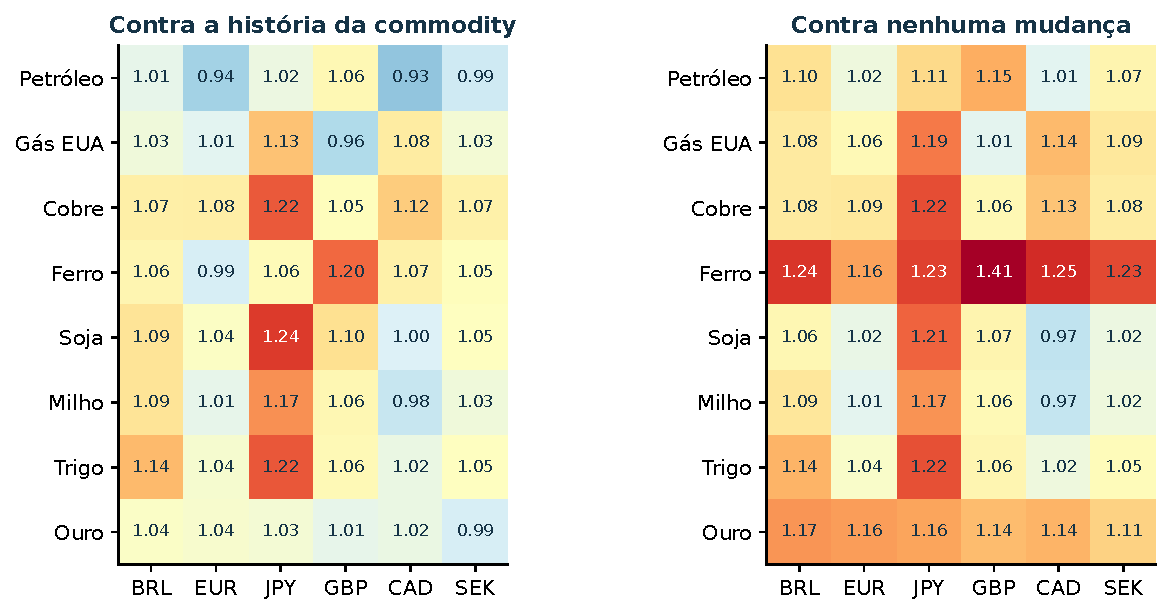
\includegraphics[width=.98\linewidth]{figures/single_currency.pdf}\caption{Preços nominais, horizonte de 12 meses à frente da origem. Cada célula é uma regressão própria; valores abaixo de 1 são melhora. O preço global de uma commodity não é replicado como seis realizações independentes.}\end{figure}
\small\begin{center}\begin{tabular}{lrr}\toprule
Commodity / moeda & RMSE / história & RMSE / sem mudança \\ \midrule
Petróleo / CAD & 0,928 & 1,005 \\
Gás EUA / GBP & 0,956 & 1,007 \\
Milho / CAD & 0,977 & 0,975 \\
Soja / CAD & 0,999 & 0,971 \\
\bottomrule\end{tabular}\end{center}\normalsize

O caso CAD $\rightarrow$ petróleo melhora o erro da regressão histórica em 7,2\%, mas fica ligeiramente pior que nenhuma mudança. Isso ilustra por que a escolha do benchmark altera a interpretação. Milho/CAD e soja/CAD têm ganhos pontuais frente a nenhuma mudança, sem evidência robusta após as correções de multiplicidade.

Não apareceu um padrão de superioridade geral do câmbio real individual no horizonte de um ano. A presença de relações econômicas entre países e commodities não dispensa a avaliação fora da amostra.

\clearpage
\section*{3. Combinar câmbios melhora a informação?}\begin{figure}[H]\centering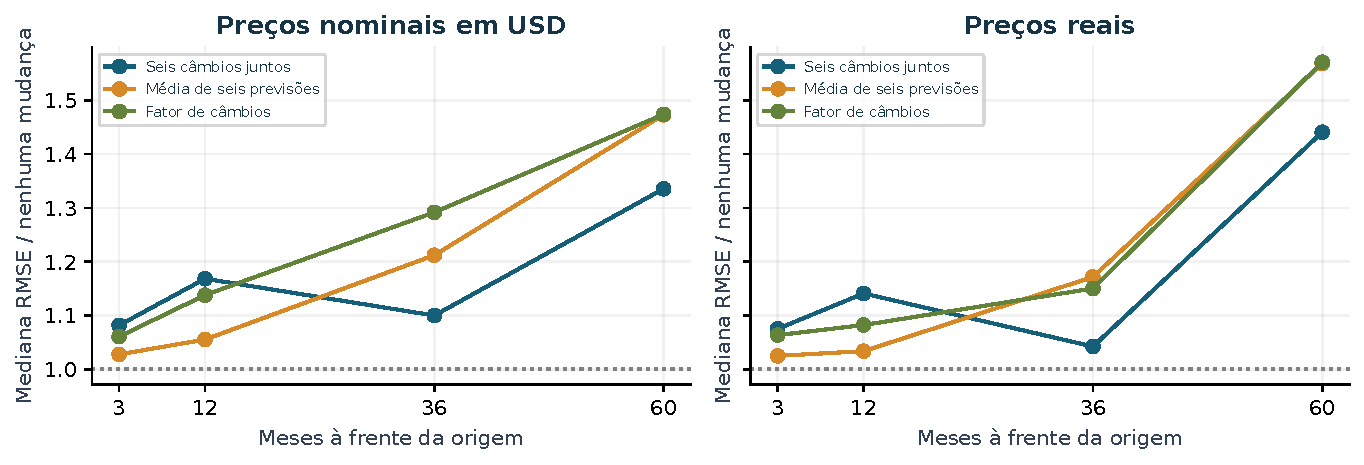
\includegraphics[width=.98\linewidth]{figures/commodity_horizons.pdf}\caption{Mediana entre as oito commodities. A mediana é resumo descritivo, não erro de uma nona commodity nem teste com oito amostras independentes.}\end{figure}
\small\begin{center}\begin{tabular}{lrrrr}\toprule
Preço & h & RMSE / história & RMSE / sem mudança & Vitórias / 8 \\ \midrule
Nominal & 3 & 1,062 & 1,082 & 0/8 \\
Nominal & 12 & 1,138 & 1,168 & 0/8 \\
Nominal & 36 & 0,816 & 1,100 & 2/8 \\
Nominal & 60 & 0,894 & 1,335 & 2/8 \\
Real & 3 & 1,023 & 1,075 & 2/8 \\
Real & 12 & 1,053 & 1,141 & 0/8 \\
Real & 36 & 0,757 & 1,042 & 2/8 \\
Real & 60 & 0,943 & 1,441 & 1/8 \\
\bottomrule\end{tabular}\end{center}\normalsize

A regressão conjunta tem mais parâmetros e pode piorar a previsão, especialmente em horizontes curtos. A média simples de previsões costuma ser menos instável. No nominal, aos 12 meses, a regressão conjunta não supera nenhuma mudança em qualquer uma das oito commodities.

Em 36 meses, o modelo conjunto melhora a história própria em sete commodities nominais e nas oito reais. Porém supera nenhuma mudança em apenas duas de cada conjunto. Uma melhora relativa grande pode ser, em parte, a correção de extrapolações ruins do benchmark histórico.

\clearpage
\section*{4--5. O componente real faz diferença?}\small\begin{center}\begin{tabular}{lrrr}\toprule
h & Informação acrescentada & Mediana / história & Mediana / sem mudança \\ \midrule
12 & Câmbio real & 1,049 & 1,088 \\
12 & Nível nominal & 1,050 & 1,092 \\
12 & Variação nominal & 1,004 & 1,039 \\
12 & Inflação relativa & 1,127 & 1,157 \\
36 & Câmbio real & 0,998 & 1,307 \\
36 & Nível nominal & 1,003 & 1,323 \\
36 & Variação nominal & 0,990 & 1,294 \\
36 & Inflação relativa & 1,041 & 1,327 \\
\bottomrule\end{tabular}\end{center}\normalsize

O nível nominal é centralizado com sua média passada; a variação nominal usa 12 meses. O componente de preços é a diferença entre Q e o log-câmbio nominal, centralizada da mesma forma. Não incluímos simultaneamente Q, nominal e preços relativos como três variáveis independentes, pois existe identidade linear entre eles.

Também estimamos história da commodity + fator comum nominal das seis moedas contra USD e, depois, acrescentamos Q individual. Esse fator é um controle empírico simples, não DXY nem um choque estrutural do dólar. A pergunta é se Q acrescenta informação além do movimento compartilhado das moedas.
\begin{figure}[H]\centering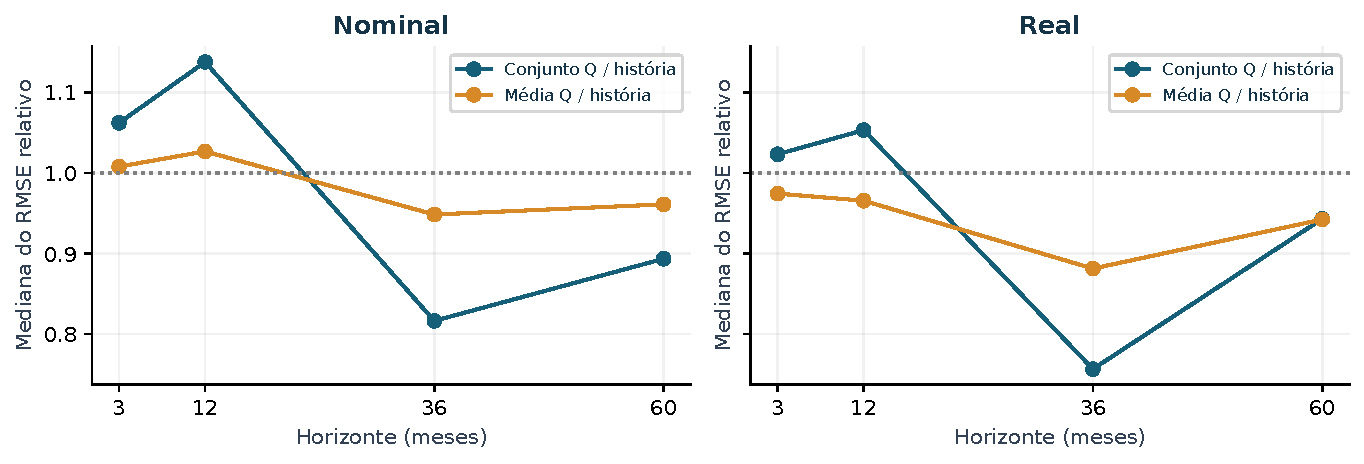
\includegraphics[width=.98\linewidth]{figures/weak_benchmark.pdf}\caption{Trocar a referência para a história própria produz uma impressão mais favorável em horizontes longos. Compare com a figura anterior, cujo benchmark é nenhuma mudança.}\end{figure}

\textbf{Deflação e disponibilidade.} No horizonte de 36 meses, a mediana do RMSE relativo à história é 0,757 para preços reais e 0,816 para nominais. Ao igualar o atraso nominal em dois meses, a mediana nominal é 0,811: a diferença não vem apenas do mês extra de disponibilidade. Isso continua sendo uma comparação descritiva entre alvos diferentes; não demonstra que o componente real ganhou conteúdo causal.

\clearpage
\section*{2 e 8. A pauta comercial organiza a previsibilidade?}\small\begin{center}\begin{tabular}{lrrrr}\toprule
Preço & h & Grupo & RMSE / história & RMSE / sem mudança \\ \midrule
Nominal & 12 & Mais expostos & 1,089 & 1,106 \\
Nominal & 12 & Demais moedas & 1,018 & 1,029 \\
Nominal & 36 & Mais expostos & 1,010 & 1,317 \\
Nominal & 36 & Demais moedas & 0,944 & 1,123 \\
Real & 12 & Mais expostos & 1,000 & 1,103 \\
Real & 12 & Demais moedas & 0,935 & 1,010 \\
Real & 36 & Mais expostos & 0,962 & 1,371 \\
Real & 36 & Demais moedas & 0,849 & 1,099 \\
\bottomrule\end{tabular}\end{center}\normalsize

Para cada grupo de commodities, as duas moedas com maior peso comercial absoluto em 1994--1996 são consideradas mais expostas. Exposição importadora também pode ser informativa: não se restringe o grupo a exportadores. As previsões individuais recebem pesos iguais dentro de cada grupo. A regra de seleção não depende dos resultados de previsão.

O grupo mais exposto não domina os demais. Isso enfraquece uma interpretação simples segundo a qual o país mais ligado comercialmente a uma commodity necessariamente a antecipa melhor. O grupo pode conter um grande importador cuja moeda incorpora muitos outros determinantes.

\textbf{Limitações concretas.} Os pesos são antigos, os quatro grupos são amplos e poucas cotações representam cada cesta. O Brasil, por exemplo, apresenta peso negativo em energia na janela histórica, o que não pretende descrever sua pauta atual. Alemanha é somente uma aproximação para EUR. Ouro não tem cobertura adequada pela participação de minérios/metais usada aqui; por isso foi excluído desta comparação econômica de grupos, embora suas previsões permaneçam na grade geral.

\textbf{Na direção inversa.} Substituir uma cesta global pela proxy comercial nacional, sem Q, reduziu parte do erro em horizontes longos em relação ao modelo global, mas não estabeleceu superioridade sobre nenhuma mudança. O maior interesse aparece ao decompor a proxy comercial em movimento global e específico, discutido a seguir.

\textbf{O que este teste não faz.} Não estima elasticidade de exportação, não usa os pesos como instrumento e não mede renda gerada por um choque. A associação entre preços internacionais e câmbio pode continuar refletindo atividade e condições financeiras comuns.

\clearpage
\section*{6--7. Commodities acrescentam informação ao EJR?}\small\begin{center}\begin{tabular}{lrrrr}\toprule
Extensão / EJR & 3m & 12m & 36m & 60m \\ \midrule
EJR + preço global & 0,999 & 1,015 & 1,005 & 0,979 \\
EJR + cesta comercial & 1,002 & 1,003 & 1,010 & 1,015 \\
EJR + global e variação & 1,008 & 1,010 & 1,014 & 0,976 \\
EJR + interação global & 1,011 & 1,031 & 1,014 & 0,980 \\
EJR + interação comercial & 1,007 & 1,030 & 1,030 & 1,055 \\
EJR + exposição heterogênea & 1,000 & 1,028 & 1,031 & 0,990 \\
EJR + componente específico & 1,005 & 1,020 & 0,918 & 0,858 \\
\bottomrule\end{tabular}\end{center}\normalsize

Razão entre RMSE da extensão e RMSE de EJR, nas mesmas origens. As extensões mantêm a restrição de intercepto do modelo original. Os preços entram deflacionados e conhecidos com dois meses de atraso. Momentum é a variação de 12 meses. O h de 60 meses do modelo com momentum tem início mais tardio por necessidade de treino; a comparação permanece pareada.

Nos horizontes curtos, a maior parte das inclusões piora ou altera muito pouco o resultado. Preço global e cesta comercial isolados não resolvem a previsibilidade cambial. O componente específico se destaca em 36 e 60 meses, mas não nos horizontes curtos.
\subsection*{Comparação com nenhuma mudança}
\small\begin{center}\begin{tabular}{lrrrr}\toprule
Modelo / sem mudança & 3m & 12m & 36m & 60m \\ \midrule
EJR original & 1,011 & 1,039 & 1,096 & 1,037 \\
EJR + específico & 1,016 & 1,059 & 1,006 & 0,890 \\
\bottomrule\end{tabular}\end{center}\normalsize

Em 36 meses, a extensão específica melhora EJR, mas ainda tem erro agregado ligeiramente maior que nenhuma mudança. Em 60 meses, supera ambos na amostra integral. Essa é a principal descoberta exploratória deste estudo.

\textbf{Teste comparável.} A extensão restrita é $\widehat{\Delta_h s}_{i,t}=\beta_h Q_{i,t}+\gamma_h Z_{i,t}$, ou sua versão com mais componentes. As médias para centralizar níveis são estimadas com a informação disponível até $t$, como no EJR. Nenhum intercepto adicional é introduzido. A auditoria reproduz numericamente EJR quando as colunas de commodities são removidas.

\textbf{Commodities sozinhas.} Nos modelos flexíveis, nível e variação global sem Q tiveram RMSE sobre nenhuma mudança de 1,031; 1,102; 1,515; 1,753 nos quatro horizontes. A cesta comercial isolada ficou em 1,012; 1,057; 1,275; 1,371. São resultados desfavoráveis, não evidência de uma alternativa autossuficiente ao sinal real.

\clearpage

\section*{10. O que significa o componente específico?}
Seja $b_{k,t}$ o log-preço real conhecido do setor $k$. Definimos
\[ G_t=\frac{1}{4}\sum_k b_{k,t},\qquad Z_{i,t}=\sum_k w_{ik}b_{k,t},\qquad e_i=\sum_k w_{ik}. \]
O componente específico é
\[ Z^{esp}_{i,t}=Z_{i,t}-e_iG_t=\sum_k w_{ik}(b_{k,t}-G_t). \]
Ele distingue, por exemplo, um movimento concentrado em metais de uma alta comum a todas as cestas. A regressão inclui Q, o componente global e o específico. Todos os níveis são centralizados com médias disponíveis na origem.

Essa decomposição não extrai um choque estrutural. É uma forma transparente de separar informação comum e composição comercial. Seus pesos não são escolhidos para maximizar a previsão.
\begin{figure}[H]\centering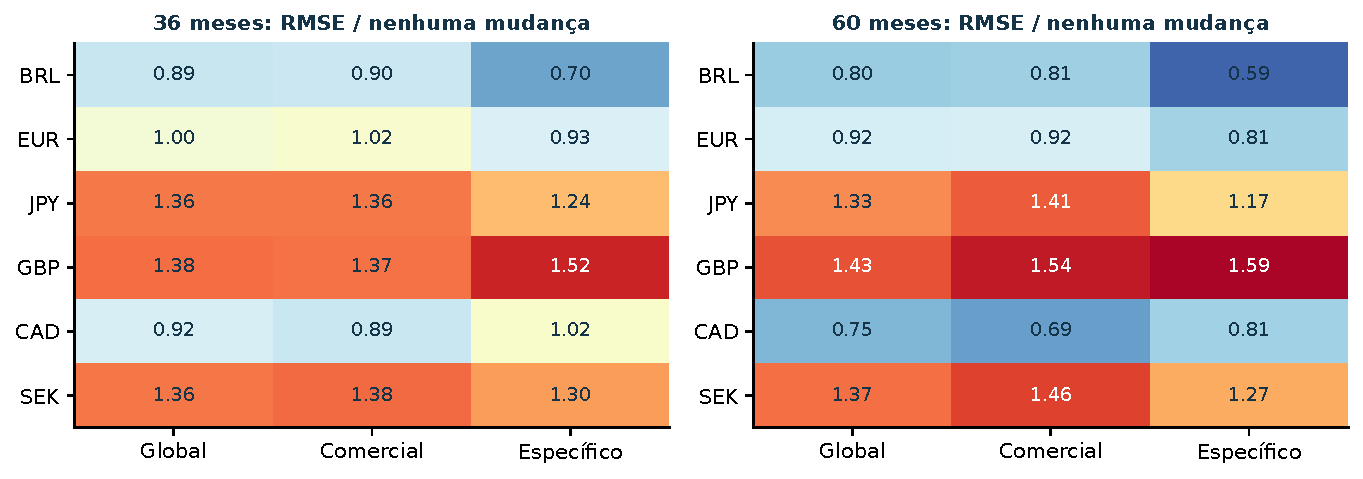
\includegraphics[width=.98\linewidth]{figures/fx_countries.pdf}\caption{RMSE sobre nenhuma mudança por moeda. O ganho agregado em cinco anos não é uniforme: BRL, EUR e CAD ficam abaixo de 1; JPY, GBP e SEK ficam acima.}\end{figure}

CAD já era bem previsto pelo EJR nesta janela: acrescentar o específico piora seu erro relativo a EJR, embora continue melhor que nenhuma mudança. Já BRL apresenta melhora relevante nas duas comparações. Assim, ``melhor que nenhuma mudança'' e ``commodities acrescentaram valor ao EJR'' são perguntas diferentes também dentro de cada país.

\clearpage
\section*{Onde está a melhora e onde o modelo erra}\small\begin{center}\begin{tabular}{lrr}\toprule
Moeda, horizonte 60m & RMSE / EJR & RMSE / sem mudança \\ \midrule
BRL & 0,739 & 0,585 \\
EUR & 0,907 & 0,815 \\
JPY & 0,852 & 1,175 \\
GBP & 1,032 & 1,586 \\
CAD & 1,146 & 0,812 \\
SEK & 0,887 & 1,272 \\
\bottomrule\end{tabular}\end{center}\normalsize
\begin{figure}[H]\centering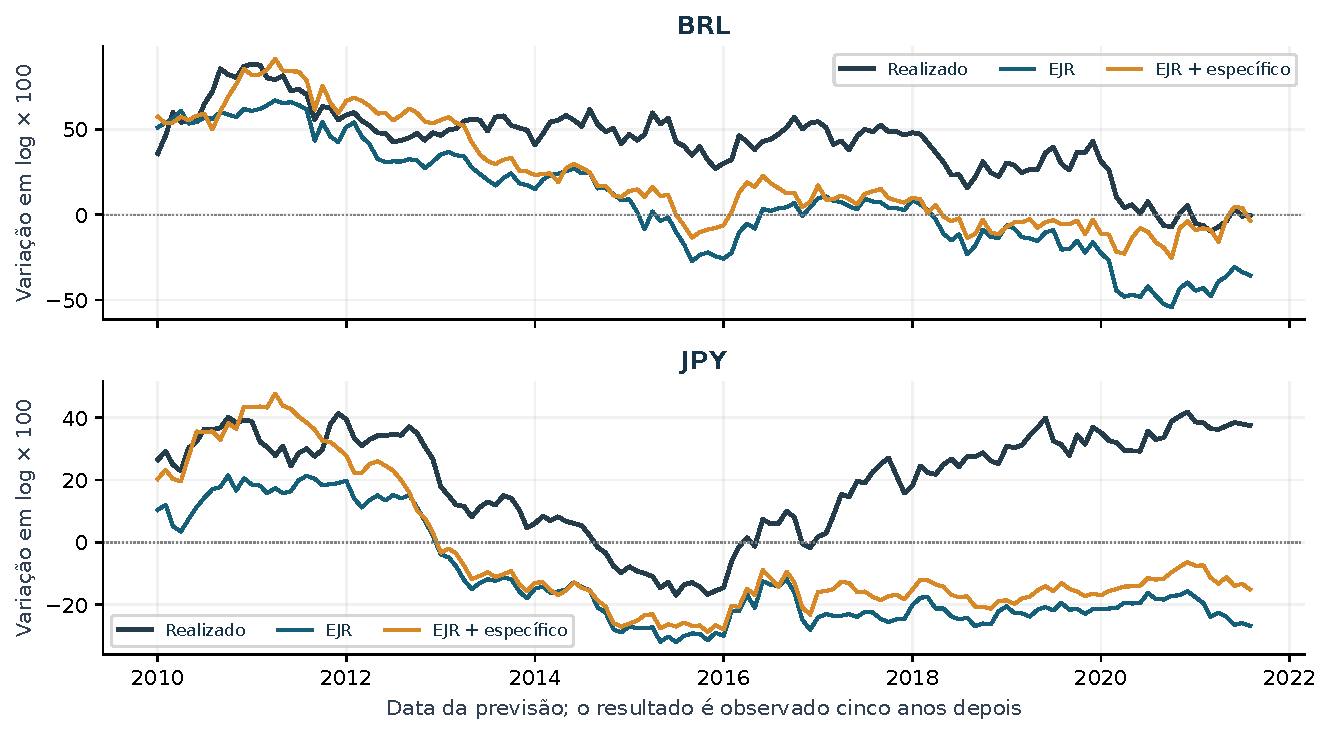
\includegraphics[width=.98\linewidth]{figures/forecast_examples.pdf}\caption{Exemplos escolhidos para mostrar heterogeneidade: BRL, com melhora, e JPY, com erro persistente. O eixo horizontal é a origem, não o mês de realização. Cada ponto usa uma previsão distinta de cinco anos; as janelas se sobrepõem.}\end{figure}

O erro agregado é calculado agrupando previsões em log, sem padronizar cada moeda pela sua volatilidade. Portanto moedas com variações maiores, como BRL nesta amostra, têm influência maior sobre o RMSE agregado. A exclusão de BRL é essencial para interpretar a descoberta; não basta contar quantos países tiveram melhora.

\clearpage
\section*{A descoberta sobrevive a variações razoáveis?}\begin{figure}[H]\centering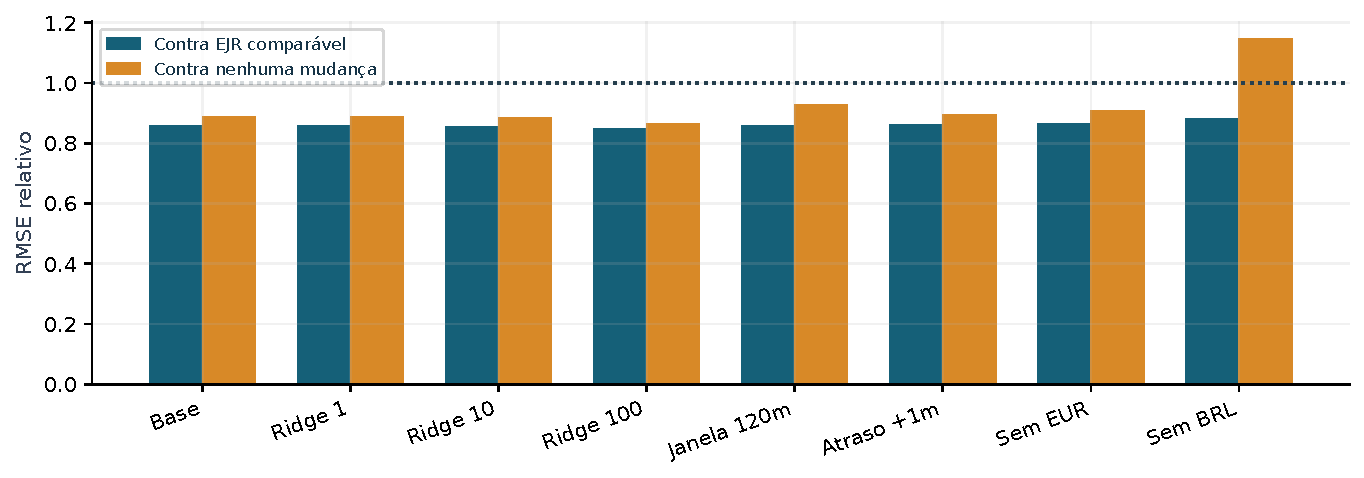
\includegraphics[width=.98\linewidth]{figures/specific_robustness.pdf}\caption{Extensão específica em 60 meses. Nos testes de penalização/janela/universo, o EJR de referência recebe a mesma alteração; o benchmark de nenhuma mudança permanece explícito.}\end{figure}
\small\begin{center}\begin{tabular}{lrr}\toprule
Variação & RMSE / EJR comparável & RMSE / sem mudança \\ \midrule
base & 0,858 & 0,890 \\
ridge1 & 0,858 & 0,890 \\
ridge10 & 0,857 & 0,886 \\
ridge100 & 0,850 & 0,865 \\
rolling120 & 0,860 & 0,928 \\
lag\_extra1 & 0,862 & 0,894 \\
no\_EUR & 0,867 & 0,907 \\
no\_BRL & 0,882 & 1,147 \\
\bottomrule\end{tabular}\end{center}\normalsize

A melhora frente a EJR persiste com penalizações 1/10/100, janela móvel de 120 meses, atraso adicional das commodities e retirada de EUR ou BRL. Mas, sem BRL, o RMSE passa a 1,147 vezes o de nenhuma mudança. O resultado agregado não é transferível automaticamente ao conjunto dos demais países.

\textbf{Estabilidade temporal.} Nas origens desde 2019, restam apenas 32 previsões de cinco anos, realizadas até agosto de 2026. A razão contra EJR é 0,825, mas contra nenhuma mudança é 1,630. A extensão corrige parte de um modelo-base ruim nesse trecho; não supera uma referência simples.

Excluir alvos que atravessam 2020--2021 deixa somente 60 origens de cinco anos. Esse diagnóstico tem forte seleção de períodos e não substitui uma validação externa. Todas as sensibilidades dos demais modelos e commodities permanecem nos arquivos completos.

\clearpage
\section*{O que os intervalos e a sobreposição permitem dizer}\small\begin{center}\begin{tabular}{lrrr}\toprule
h & Referência & Ganho médio de perda & IC bootstrap 95\% \\ \midrule
36 & EJR & 0,0064 & [0,0012; 0,0112] \\
36 & RW & -0,0004 & [-0,0206; 0,0237] \\
60 & EJR & 0,0188 & [0,0091; 0,0282] \\
60 & RW & 0,0138 & [-0,0321; 0,0626] \\
\bottomrule\end{tabular}\end{center}\normalsize

Ganho positivo significa redução da perda quadrática média, em unidades de log ao quadrado. Bootstrap por datas, mantendo os choques comuns entre moedas, com 1.999 reamostragens e blocos de $h+2$ meses. Também calculamos blocos de 12 meses. Os intervalos são condicionais às previsões estimadas e não corrigem a seleção posterior do candidato.

Frente a EJR, os intervalos são favoráveis. Frente a nenhuma mudança, incluem zero. No horizonte de cinco anos há somente 140 datas sobrepostas, cerca de 2,3 blocos de 62 meses; nem um intervalo bootstrap estreito transformaria esse histórico em muitas experiências independentes.
\begin{figure}[H]\centering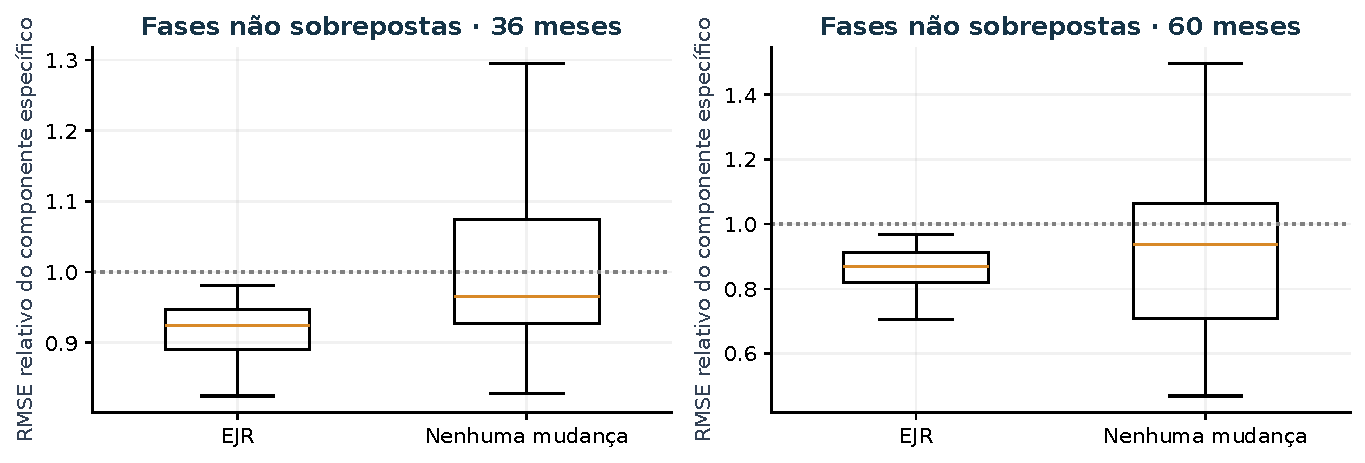
\includegraphics[width=.98\linewidth]{figures/nonoverlap.pdf}\caption{Todas as fases de seleção de origens espaçadas por h+2 meses. Cada fase contém apenas 4--5 datas para 36m e 2--3 para 60m. Não escolhemos a fase mais favorável.}\end{figure}

Em cinco anos, as razões contra nenhuma mudança variam de aproximadamente 0,47 a 1,50 conforme a fase; contra EJR, de 0,71 a 0,97. Há evidência descritiva consistente de melhora relativa a EJR, mas a superioridade contra nenhuma mudança é muito menos estável.

\textbf{P-valores.} Diferenças de perda são agregadas por data antes do HAC, com $h+2$ defasagens. Não emitimos p-valor com menos de 36 datas ou três blocos do horizonte. Holm inclui os testes contra a base e contra nenhuma mudança, nos três blocos de hipóteses. Os resultados de cinco anos permanecem descritivos.

\clearpage
\section*{11--13. Interações, referência de equilíbrio e heterogeneidade}\footnotesize\begin{center}\begin{tabular}{lrrr}\toprule
Especificação / sua base & 12m & 36m & 60m \\ \midrule
Interação global, restrita & 1,031 & 1,014 & 0,980 \\
Interação comercial, restrita & 1,030 & 1,030 & 1,055 \\
Exposição heterogênea, restrita & 1,028 & 1,031 & 0,990 \\
Referência condicional, flexível & 0,999 & 1,011 & 1,018 \\
Exposição heterogênea, flexível & 1,034 & 1,082 & 1,071 \\
\bottomrule\end{tabular}\end{center}\normalsize

\textbf{Interação.} O modelo contém $Q$, o preço global $G$ e $QG$, centralizados de acordo com a informação disponível. Isso permite que a inclinação preditiva em Q dependa do estado das commodities. Outra versão troca G pela proxy comercial. A melhora preditiva não foi geral: a interação comercial piorou EJR nos quatro horizontes, e a global permaneceu pior que nenhuma mudança.

Um coeficiente de interação não identifica a velocidade causal de convergência. Ele apenas permite uma relação condicional diferente e pergunta se essa flexibilidade prevê melhor. Nesta implementação, a complexidade adicional não foi recompensada de maneira consistente.

\textbf{Referência de equilíbrio condicional.} Primeiro projetamos Q no índice comercial e nos interceptos de país usando somente a amostra de treino; depois usamos o resíduo para prever câmbio. A hipótese é que uma parcela do desvio real possa acompanhar fundamentos de commodities. Esse procedimento impõe uma restrição de previsão; não estima um equilíbrio estrutural nem prova cointegração.

Comparado à regressão Q com os mesmos interceptos e regularização, o resíduo teve mudanças mínimas em 12 meses e piora em 36/60 meses. Acrescentar a proxy disponível não resolveu a dificuldade de distinguir desalinhamento de mudança de fundamentos.

\textbf{Exportadores e importadores.} A exposição líquida $e_i$ modifica a resposta ao global; na família flexível também modifica a inclinação em Q. Trata-se de heterogeneidade contínua, sem separar retrospectivamente países pelos resultados. A família não superou a referência simples de forma geral.

\textbf{Limite econômico.} Pesos fixos de três anos antigos, quatro cestas e seis moedas podem ser insuficientes para descrever mudanças estruturais de comércio. A ausência de ganho neste exercício não rejeita a hipótese de que fundamentos alterem o câmbio de equilíbrio; rejeita apenas a ideia de que estas especificações entregaram melhora preditiva robusta.

\clearpage
\section*{14. O ajuste aparece no câmbio ou na inflação?}\begin{figure}[H]\centering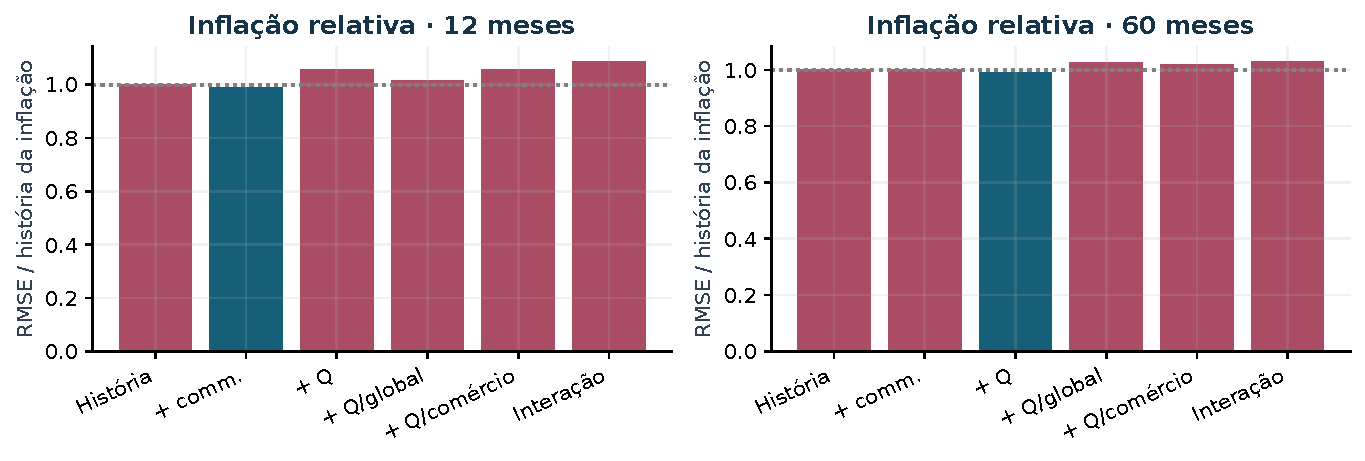
\includegraphics[width=.98\linewidth]{figures/inflation.pdf}\caption{A história própria é a referência exigente para inflação. Nenhuma mudança é mais fácil de superar quando diferenças de inflação são persistentes.}\end{figure}
\small\begin{center}\begin{tabular}{lrrr}\toprule
h & Modelo & RMSE / história & RMSE / inflação zero \\ \midrule
3 & História própria & 1,000 & 0,911 \\
3 & História + commodities & 0,998 & 0,909 \\
3 & História + Q + global & 1,019 & 0,929 \\
12 & História própria & 1,000 & 0,793 \\
12 & História + commodities & 0,988 & 0,783 \\
12 & História + Q + global & 1,015 & 0,804 \\
36 & História própria & 1,000 & 0,713 \\
36 & História + commodities & 0,998 & 0,712 \\
36 & História + Q + global & 1,109 & 0,791 \\
60 & História própria & 1,000 & 0,630 \\
60 & História + commodities & 1,001 & 0,631 \\
60 & História + Q + global & 1,025 & 0,646 \\
\bottomrule\end{tabular}\end{center}\normalsize

Commodities acrescentadas à inflação passada reduziram o erro agregado em aproximadamente 1,2\% em 12 meses, quase não alteraram 3/36 meses e pioraram ligeiramente 60 meses. O ganho incremental não se mostrou robusto após multiplicidade. Superar inflação zero é sobretudo mérito da história própria, não da commodity.

Os resultados não permitem concluir causalmente por qual canal o câmbio real se ajusta. A identidade entre câmbio nominal, preços relativos e câmbio real não identifica choques. A evidência preditiva desta extensão é mais interessante no câmbio nominal de alguns países e horizontes do que no incremento de previsão da inflação.

\clearpage

\section*{15. Direção, horizonte e interpretação da descoberta}
\textbf{Nos horizontes curtos,} de três e doze meses, os seis câmbios reais não produziram uma melhora geral nas previsões de commodities. Adicionar commodities ao EJR também não resolveu a previsão cambial. São resultados compatíveis com pouca informação incremental útil nestas especificações, não uma demonstração universal de imprevisibilidade.

\textbf{Em três anos,} câmbios conjuntos frequentemente corrigem erros da regressão baseada na história da commodity, mas raramente superam nenhuma mudança. Na direção commodities $\rightarrow$ câmbio, o componente específico melhora EJR, porém o RMSE agregado ainda fica ligeiramente acima da referência simples.

\textbf{Em cinco anos,} o componente específico é o candidato mais interessante. Ele melhora o EJR e, na amostra integral, supera nenhuma mudança. A falta de estabilidade sem BRL e nas origens recentes, além do reduzido número de episódios independentes, impede declarar previsibilidade geral comprovada.

\textbf{Não há simetria automática.} Uma variável ajudar a prever outra em determinada especificação não implica a relação inversa, nem uma cadeia causal. Commodities são médias mensais com atraso de divulgação, enquanto o câmbio é fechamento mensal. Os alvos de commodities também têm bases conhecidas em $t-1$ ou $t-2$; os h não são intervalos idênticos desde o último preço observado.

\textbf{A contribuição mais defensável para o trabalho.} Mostrar que decompor a informação de commodities em global e composição comercial pode melhorar uma previsão EJR específica, sem confundir isso com superar todos os benchmarks. Essa pergunta é menor e mais precisa do que afirmar que commodities e câmbio se antecipam de forma generalizada.

\textbf{Próxima hipótese a congelar.} Manter Q, fator global e componente comercial específico, com a mesma definição de dados e pesos, e avaliar em dados novos ou em outro universo de países escolhido previamente. Uma ampliação para as moedas exportadoras estudadas por Chen--Rogoff--Rossi seria uma validação externa relevante; ela não foi simulada como se já tivesse sido executada neste relatório.

O presente estudo inclui seis moedas da replicação anterior, não o universo completo do artigo de commodities. A unidade do trabalho continua sendo a previsão macroeconômica, sem conversão dos resultados em recomendação financeira.

\clearpage
\section*{Auditoria, disponibilidade e limites dos dados}\textbf{36 verificações de integridade passaram.} 
Foram conferidos: equivalência do EJR restrito ao original; invariância ao truncar o futuro nos modelos regular, PCA, interação e referência condicional; invariância das previsões antigas ao corromper rótulos e preditores futuros; identidade do câmbio real; calendário e preços; pesos anteriores à estimação; ausência de índices oficiais com pesos futuros; hashes de fontes; unicidade das previsões e preservação dos dois estudos anteriores.

\textbf{Disponibilidade.} A trilha registra o primeiro e último mês de treino e quando o último alvo ficou disponível. Todas as datas admitidas são anteriores à origem. Commodity nominal usa um mês de atraso e real usa dois; CPI tem dois meses. Isso disciplina a cronologia, mas não reconstrói todos os vintages históricos. Revisões nas séries e nos dados comerciais ainda podem afetar o que um pesquisador realmente teria observado.

\textbf{Uma inconsistência documental foi examinada.} O XLSX contém uma aba de diferenças, incluindo soja de julho de 2026 com dois valores. Usamos 478 USD/t da aba Monthly Prices, confirmado no PDF oficial da Pink Sheet de setembro de 2026 [4]. Os arquivos brutos são preservados. As demais cotações selecionadas não apareceram nessa lista de diferenças.

\textbf{Mudanças de definição.} As descrições da própria fonte registram alterações de qualidade/local de entrega e de tipo de cotação, inclusive em soja, trigo e ferro. O passado do ferro contém referências contratuais e a série selecionada é apresentada como cfr spot; isso exige cautela com a homogeneidade do histórico. A fonte não foi tratada como um contrato financeiro imutável.

\textbf{Quantidade não é identificação.} O arquivo tem muitas previsões porque cruza modelos, moedas, commodities e horizontes. Isso não cria novas realizações macroeconômicas. A análise de uma commodity não repete o mesmo alvo em seis linhas para inflar o tamanho da amostra. No painel cambial, as perdas são agregadas por data antes da inferência.

\textbf{Comparações múltiplas.} Só um ganho incremental com p Holm abaixo de 5\% permaneceu na grade principal: Q do euro condicionado ao fator nominal comum, para milho real em 36 meses, contra o benchmark que já contém o fator dólar. Seu RMSE foi 1,124 vezes o de nenhuma mudança, e não o superou estatisticamente. Um p pequeno relativo a uma base específica não equivale a sucesso geral de previsão.

Os intervalos dos candidatos são pós-seleção, condicionais às previsões e não constituem inferência de uma réplica exata do bootstrap dos artigos. Resultados longos são apresentados como evidência exploratória, com suas limitações efetivas.

\clearpage
\section*{Apêndice A. Grade de commodities: nominal}Conjunto = seis Q na regressão; média = seis previsões individuais.\par \footnotesize\begin{center}\begin{tabular}{lrrrrrr}\toprule
Alvo & h & Datas & Conj./hist. & Conj./RW & Média/hist. & Média/RW \\ \midrule
Petróleo & 3 & 197 & 1,006 & 1,030 & 0,957 & 0,980 \\
Petróleo & 12 & 188 & 1,056 & 1,145 & 0,955 & 1,034 \\
Petróleo & 36 & 164 & 0,819 & 1,013 & 0,895 & 1,108 \\
Petróleo & 60 & 140 & 1,008 & 1,672 & 0,962 & 1,595 \\
Gás EUA & 3 & 197 & 1,019 & 1,054 & 0,991 & 1,025 \\
Gás EUA & 12 & 188 & 0,981 & 1,034 & 1,005 & 1,060 \\
Gás EUA & 36 & 164 & 0,729 & 1,199 & 0,969 & 1,595 \\
Gás EUA & 60 & 140 & 0,966 & 2,172 & 0,968 & 2,177 \\
Cobre & 3 & 197 & 1,194 & 1,214 & 1,033 & 1,050 \\
Cobre & 12 & 188 & 1,081 & 1,089 & 1,053 & 1,061 \\
Cobre & 36 & 164 & 0,814 & 1,165 & 0,953 & 1,364 \\
Cobre & 60 & 140 & 0,943 & 1,792 & 0,961 & 1,825 \\
Ferro & 3 & 197 & 1,082 & 1,126 & 1,000 & 1,040 \\
Ferro & 12 & 188 & 1,343 & 1,570 & 1,037 & 1,212 \\
Ferro & 36 & 164 & 0,783 & 0,978 & 0,925 & 1,156 \\
Ferro & 60 & 140 & 0,904 & 1,338 & 0,913 & 1,352 \\
Soja & 3 & 197 & 1,026 & 1,036 & 1,008 & 1,018 \\
Soja & 12 & 188 & 1,434 & 1,395 & 1,057 & 1,028 \\
Soja & 36 & 164 & 0,910 & 1,070 & 0,931 & 1,095 \\
Soja & 60 & 140 & 0,666 & 0,999 & 0,748 & 1,122 \\
Milho & 3 & 197 & 1,049 & 1,073 & 1,008 & 1,030 \\
Milho & 12 & 188 & 1,195 & 1,192 & 1,017 & 1,014 \\
Milho & 36 & 164 & 0,841 & 1,130 & 0,944 & 1,268 \\
Milho & 60 & 140 & 0,574 & 0,883 & 0,769 & 1,185 \\
Trigo & 3 & 197 & 1,077 & 1,091 & 1,012 & 1,025 \\
Trigo & 12 & 188 & 1,364 & 1,371 & 1,045 & 1,051 \\
Trigo & 36 & 164 & 1,042 & 0,982 & 0,982 & 0,925 \\
Trigo & 60 & 140 & 0,883 & 1,126 & 0,967 & 1,233 \\
Ouro & 3 & 197 & 1,075 & 1,103 & 1,018 & 1,044 \\
Ouro & 12 & 188 & 1,006 & 1,128 & 1,016 & 1,139 \\
Ouro & 36 & 164 & 0,790 & 1,315 & 0,984 & 1,637 \\
Ouro & 60 & 140 & 0,630 & 1,333 & 0,980 & 2,074 \\
\bottomrule\end{tabular}\end{center}\normalsize

Valores menores que 1 indicam melhora. Datas são origens com alvo realizado e modelos pareados; não são episódios independentes. O arquivo completo inclui Q individual, nominal em nível/variação, preços relativos, controle dólar, fatores e grupos comerciais, além do período recente. Não há ajuste de uma estratégia financeira.

\clearpage
\section*{Apêndice A. Grade de commodities: real}Conjunto = seis Q na regressão; média = seis previsões individuais.\par \footnotesize\begin{center}\begin{tabular}{lrrrrrr}\toprule
Alvo & h & Datas & Conj./hist. & Conj./RW & Média/hist. & Média/RW \\ \midrule
Petróleo & 3 & 195 & 0,912 & 0,963 & 0,882 & 0,932 \\
Petróleo & 12 & 186 & 0,939 & 1,046 & 0,874 & 0,974 \\
Petróleo & 36 & 162 & 0,765 & 1,036 & 0,863 & 1,169 \\
Petróleo & 60 & 138 & 1,015 & 1,836 & 0,964 & 1,743 \\
Gás EUA & 3 & 195 & 1,014 & 1,072 & 0,983 & 1,039 \\
Gás EUA & 12 & 186 & 0,950 & 1,032 & 1,001 & 1,088 \\
Gás EUA & 36 & 162 & 0,734 & 1,328 & 0,957 & 1,731 \\
Gás EUA & 60 & 138 & 0,953 & 2,302 & 0,962 & 2,324 \\
Cobre & 3 & 195 & 1,214 & 1,246 & 0,999 & 1,026 \\
Cobre & 12 & 186 & 1,030 & 1,068 & 0,989 & 1,025 \\
Cobre & 36 & 162 & 0,728 & 1,227 & 0,837 & 1,411 \\
Cobre & 60 & 138 & 1,008 & 2,281 & 0,973 & 2,203 \\
Ferro & 3 & 195 & 1,046 & 1,127 & 0,967 & 1,042 \\
Ferro & 12 & 186 & 1,219 & 1,452 & 0,994 & 1,184 \\
Ferro & 36 & 162 & 0,742 & 0,941 & 0,884 & 1,121 \\
Ferro & 60 & 138 & 0,934 & 1,409 & 0,923 & 1,393 \\
Soja & 3 & 195 & 0,950 & 1,000 & 0,940 & 0,990 \\
Soja & 12 & 186 & 1,218 & 1,313 & 0,922 & 0,994 \\
Soja & 36 & 162 & 0,823 & 1,001 & 0,852 & 1,036 \\
Soja & 60 & 138 & 0,762 & 1,232 & 0,780 & 1,262 \\
Milho & 3 & 195 & 1,007 & 1,052 & 0,969 & 1,012 \\
Milho & 12 & 186 & 1,077 & 1,116 & 0,939 & 0,974 \\
Milho & 36 & 162 & 0,790 & 1,048 & 0,885 & 1,174 \\
Milho & 60 & 138 & 0,813 & 0,946 & 0,765 & 0,890 \\
Trigo & 3 & 195 & 1,033 & 1,079 & 0,980 & 1,024 \\
Trigo & 12 & 186 & 1,154 & 1,275 & 0,942 & 1,042 \\
Trigo & 36 & 162 & 0,912 & 0,943 & 0,879 & 0,908 \\
Trigo & 60 & 138 & 0,952 & 1,283 & 0,964 & 1,299 \\
Ouro & 3 & 195 & 1,093 & 1,150 & 1,023 & 1,077 \\
Ouro & 12 & 186 & 1,006 & 1,166 & 1,030 & 1,194 \\
Ouro & 36 & 162 & 0,748 & 1,425 & 0,954 & 1,818 \\
Ouro & 60 & 138 & 0,554 & 1,472 & 0,915 & 2,432 \\
\bottomrule\end{tabular}\end{center}\normalsize

Valores menores que 1 indicam melhora. Datas são origens com alvo realizado e modelos pareados; não são episódios independentes. O arquivo completo inclui Q individual, nominal em nível/variação, preços relativos, controle dólar, fatores e grupos comerciais, além do período recente. Não há ajuste de uma estratégia financeira.

\clearpage
\section*{Apêndice B. Toda a grade cambial contra nenhuma mudança}\footnotesize\begin{center}\begin{tabular}{lrrrr}\toprule
Modelo / RW & 3m & 12m & 36m & 60m \\ \midrule
RW & 1,000 & 1,000 & 1,000 & 1,000 \\
EJR & 1,011 & 1,039 & 1,096 & 1,037 \\
AR & 1,010 & 1,026 & 1,194 & 1,394 \\
Q & 1,009 & 1,033 & 1,294 & 1,581 \\
Commodity & 1,031 & 1,102 & 1,515 & 1,753 \\
Trade\_only & 1,012 & 1,057 & 1,275 & 1,371 \\
Q\_Global & 1,020 & 1,044 & 1,333 & 1,654 \\
Q\_Momentum & 1,028 & 1,100 & 1,459 & 1,705 \\
Q\_GlobalMom & 1,035 & 1,119 & 1,568 & 1,849 \\
Q\_Trade & 1,011 & 1,034 & 1,284 & 1,518 \\
Q\_TradeMom & 1,019 & 1,082 & 1,374 & 1,606 \\
Q\_Interaction & 1,043 & 1,100 & 1,336 & 1,581 \\
Q\_TradeInteraction & 1,014 & 1,032 & 1,318 & 1,517 \\
Q\_Exposure & 1,036 & 1,068 & 1,401 & 1,694 \\
Q\_Specific & 1,025 & 1,052 & 1,262 & 1,477 \\
Q\_Equilibrium & 1,009 & 1,032 & 1,308 & 1,609 \\
REJR\_Global & 1,010 & 1,054 & 1,102 & 1,015 \\
REJR\_Trade & 1,013 & 1,042 & 1,108 & 1,053 \\
REJR\_GlobalMom & 1,019 & 1,049 & 1,112 & 1,054 \\
REJR\_Interaction & 1,023 & 1,071 & 1,112 & 1,017 \\
REJR\_TradeInteraction & 1,019 & 1,070 & 1,130 & 1,095 \\
REJR\_Exposure & 1,011 & 1,067 & 1,131 & 1,027 \\
REJR\_Specific & 1,016 & 1,059 & 1,006 & 0,890 \\
\bottomrule\end{tabular}\end{center}\normalsize

\texttt{REJR}: extensão estrita da replicação sem intercepto; \texttt{Q}: regressão flexível com efeitos por país e ridge. \texttt{Global}: cesta global real; \texttt{Trade}: proxy comercial; \texttt{Specific}: componente comercial líquido do global. \texttt{Mom}: variação de 12 meses; \texttt{Interaction}: produto com Q; \texttt{Exposure}: heterogeneidade pela exposição; \texttt{Equilibrium}: resíduo da projeção condicional. \texttt{AR} usa variação cambial passada. As datas podem diferir entre especificações devido ao treino, mas cada razão tem benchmark pareado.

Os p-valores completos, comparações adicionais contra EJR/Q, países individuais, datas iniciais/finais e janela recente estão em \texttt{tables/metrics.csv}. Todos os modelos da grade inicial foram mantidos, inclusive os que pioram fortemente os erros.

\clearpage

\section*{Fontes e reprodução}
\begin{enumerate}[leftmargin=1.7em,itemsep=7pt]
\item Eichenbaum, M.; Johannsen, B. K.; Rebelo, S. \emph{Monetary Policy and the Predictability of Nominal Exchange Rates}. NBER WP 23158, revisão de 2019; artigo e slides da aula 8 já presentes no repositório. \href{https://www.nber.org/papers/w23158}{Página do trabalho}.
\item Chen, Y.; Rogoff, K.; Rossi, B. \emph{Can Exchange Rates Forecast Commodity Prices?} Quarterly Journal of Economics, 125(3), 1145--1194, 2010. \href{https://scholar.harvard.edu/sites/scholar.harvard.edu/files/rogoff/files/125-3-1145.pdf}{Texto disponibilizado pelos autores}.
\item Chen, Rogoff e Rossi. \emph{Can Exchange Rates Forecast Commodity Prices? An Update}, fevereiro de 2014. \href{https://scholar.harvard.edu/files/rogoff/files/crr2014a.pdf}{Atualização dos autores}.
\item Banco Mundial, Commodity Markets / Pink Sheet. XLSX histórico e PDF de setembro de 2026. \href{https://www.worldbank.org/en/research/commodity-markets}{Página oficial}; \href{https://thedocs.worldbank.org/en/doc/74e8be41ceb20fa0da750cda2f6b9e4e-0050012026/related/CMO-Pink-Sheet-September-2026.pdf}{PDF conferido}. Descrições e pesos oficiais constam no próprio XLSX.
\item Banco Mundial, World Development Indicators, API pública. Participações de combustíveis, alimentos, matérias-primas agrícolas e minérios/metais nas exportações/importações, e valores totais de comércio, 1994--1996. Indicadores TX/TM.VAL.FUEL.ZS.UN, FOOD.ZS.UN, AGRI.ZS.UN, MMTL.ZS.UN e MRCH.CD.WT. \href{https://api.worldbank.org/v2/indicator/TX.VAL.FUEL.ZS.UN?format=json}{Exemplo de metadados}; URLs completas dos dez downloads no manifesto.
\item Gruss, B.; Kebhaj, S. \emph{Commodity Terms of Trade: A New Database}. IMF WP/19/21, 2019. \href{https://www.imf.org/-/media/files/publications/wp/2019/wp1921.pdf}{Metodologia}; \href{https://data.imf.org/en/datasets/IMF.RES:CTOT}{Base CTOT}. Referência metodológica; seus índices não foram usados como entradas.
\end{enumerate}

\textbf{Reprodução.} Pasta \texttt{third/}. Executar \texttt{run.ps1} na raiz do repositório para preparar os dados salvos, estimar a grade principal, rodar sensibilidades, validar e gerar a fonte/PDF. Não é necessário novo download. O Python e o Tectonic são os executáveis do projeto; não foi adicionada dependência. XLSX é lido como XML sem modificar o arquivo.

\textbf{Resultados auditáveis.} \texttt{metrics.csv} contém todas as comparações; \texttt{predictions.csv.gz}, as previsões individuais; \texttt{audit.csv}, o relógio de cada ajuste. \texttt{sensitivity.csv} e os arquivos de intervalos/fases guardam a exploração completa. \texttt{data/manifest.json} registra URLs, hashes e falhas de download dos PDFs externos, consultados na web. Dados usados na estimação foram todos baixados e preservados.

\textbf{Preservação.} Os 166 arquivos anteriores congelados no início permanecem idênticos. Os hashes, o protocolo e o registro de exploração documentam o escopo. A fonte LaTeX está incluída no pacote; as oito figuras têm versões vetoriais PDF e PNG.

\end{document}
